\chapter{Cast of Characters}

I want my text to be something you want to read. In today's hurry-up
world, students actually do not read as much as they did in the past. That is
sad, because you can learn a lot from reading a well-written text.

Yes, there are badly written textbooks around, maybe even mine!

Probably, my most favorite book is {\it{Godel, Escher, Bach}}, by Douglas Hofstader
\cite{Hofstadter:1999}. I first read this, shortly after it came out. In this
book a set of characters lay out an interesting concept in one short chapter,
then the next chapter presents that concept in terms that are now fun to read.
The normally dry text, suddenly comes to life. Douglas won a Pulitzer Prize for
this book, As a Computer Science student, you should read it! I am currently on
my seventh pass through it!

I am stealing Douglas' idea, I have my own characters, and I use them in
these lecture notes on occasion.

We will follow four characters through our journey into computers and
programming. These four are good friends, but have very different goals in
life. That affects how they approach problems they encounter.

Like all teams, they have to work through their differences and come up with an
approach to getting some job done that works for everyone.

Here are our characters:

\section{Nick:   The "Doer"}

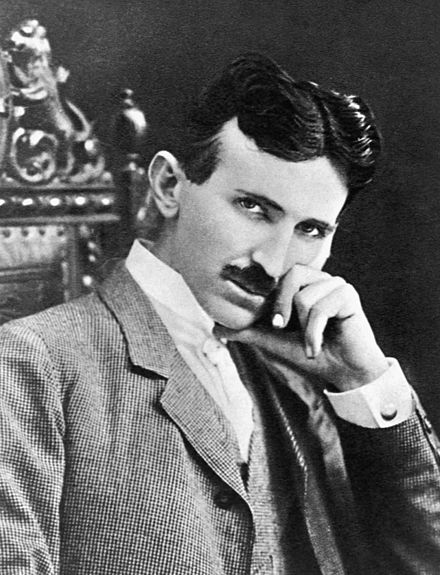
\includegraphics[width=.3\textwidth]{nikola-tesla.jpg}

Nick has a few interesting characteristics:

\begin{itemize}
    \item{Tank - impervious to harm.} 
    \item{Gets blown up a lot, but survives.}
    \item{Hates to wait for anything.}
    \item{Needs lots of documentation.}
    \item{Can fix anything.}
    \item{Mechanical genius.}
    \item{Drives a Ford Mustang (GT)}
    \item{Uses Windows 10 Pro.}
    \item{named after: Nikola Tesla}
\end{itemize}
    

\section{Ada:  Curious about everything!}
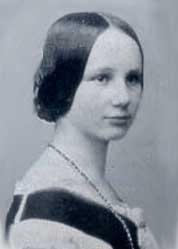
\includegraphics[width=.3\textwidth]{ada-lovelace.jpg}

Ada is going to learn as much as she can about everything. She has a burning
desire to know something about everything!

\begin{itemize}
    \item{Questions things a lot.}
    \item{Never quit asking "why" when told how something works.}
    \item{Tends to stop working on a problem when she sees the answer.}
    \item{Seems interested in everything, especially technical stuff.}
    \item{She is a peace maker, trying to calm things down when they get tense.}
    \item{Drives a Prius.}
    \item{Uses a Macbook Pro.}
    \item{Named after Ada Lovelace.}
\end{itemize}


\section{Leo: the mechanic.}

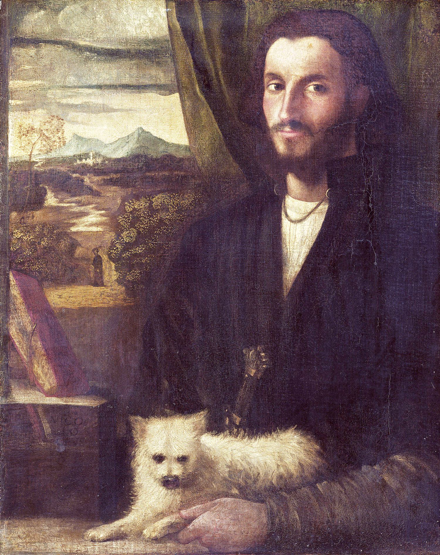
\includegraphics[width=.3\textwidth]{leonardo-da-vinci.png}

Leo is the mechanic of the bunch. He is constantly taking things apart so he
can figure out how they work. He is also an artist. As he disassembles things,
he makes drawings of the gadgets he is studying. Leo can take a box of junk and
come up with a Ferrari!

\begin{itemize}
    \item{He can see how things move, because he understands how they are put together.}
    \item{Likes to concoct new machines.}
    \item{Rube Goldberg is his idol!}
    \item{Drives a 1964 Alfa Romeo Giulia Spider sports car.}
    \item{He does not own a stinking computer!}
    \item{Named after Leonardo da Vinci.}
\end{itemize}

\section{Alan: the wizard}

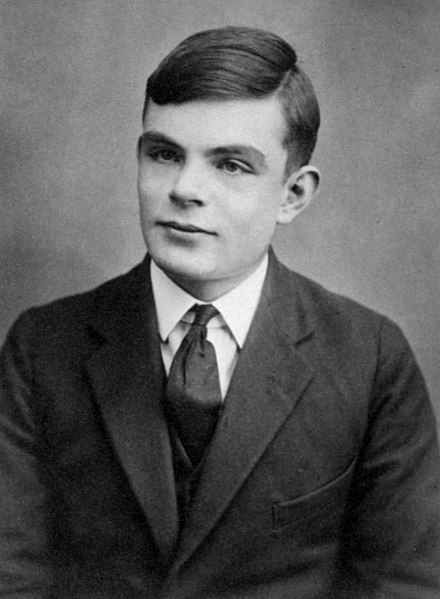
\includegraphics[width=.3\textwidth]{alan-turing.jpg}

Alan is the genius of the group. He does know a lot about everything. In fact,
tripping him up is a game the other two like to play. How he got this way is a
puzzle, but he has been caught, late at night, scouring the Internet with his
iPad!

\begin{itemize}
	\item{Comes across al very knowledgeable, even if he is not really that up on the topic.}
    \item{Has a photographic memory, seldom forgets anything.}
    \item{Wants to guide the action because he knows the "right way".}
    \item{Something of a space cadet, he wanders off track at times.}
    \item{Drives a Mercedes (he got it used)}
    \item{Uses Linux on an Alienware Laptop.}
    \item{Named after Alan Turing.}
\end{itemize}
